\documentclass[11pt]{article}
\usepackage{graphicx} % Required for inserting images
\usepackage{newtxtext} % This package sets Times New Roman as the main font
\usepackage{ragged2e} % This package is used to justify the text
\usepackage{setspace} % This package is used to set the line spacing
\usepackage[a4paper, left=3cm, top=3cm, bottom=2cm, right=2cm]{geometry} % This package is used to set the margins
\usepackage{lipsum} % This package is used to generate filler text
\usepackage{fancyhdr} % This package is used to customize the headers and footers
\usepackage{titlesec} % This package is used to customize titles
\usepackage[portuguese]{babel} % This package is used to translate the names of the document elements
\usepackage{hyperref} % This package is used to create hyperlinks in the document
\usepackage{indentfirst}
\setlength{\parindent}{1.25cm}  % This command sets the size of the indent
\usepackage{siunitx}
\sisetup{
  output-decimal-marker = {,},
  inter-unit-product = \ensuremath{{}\cdot{}},
  per-mode = symbol
}
\DeclareSIUnit{\real}{R\$}
\newcommand{\real}[1]{R\$#1}
\usepackage{float}
\usepackage{footnotehyper}


\begin{document}

\begin{titlepage}
    \centering
    \vspace*{1cm}
    \Large\textbf{INSPER – INSTITUTO DE ENSINO E PESQUISA}\\
    \Large ADMINISTRAÇÃO/ECONOMIA\\
    \vspace{1.5cm}
    \Large\textbf{ATIVIDADE PRÁTICA SUPERVISIONADA II - FINANÇAS I}\\
    \vspace{1.5cm}
    \large CAMIL\\
    Prof. Dr. Leonardo Pagano\\
    Profa. Auxiliar Cinthia Barbosa da Silva\\
    \vfill
    \normalsize
    Beatriz Emi Ueda, \href{mailto:beatrizeu@al.insper.edu.br}{beatrizeu@al.insper.edu.br}\\
    Beatriz Fernandes da Silva, \href{mailto:beatrizfs1@al.insper.edu.br}{beatrizfs1@al.insper.edu.br}\\
    Gabriela Abib, \href{mailto:gabrielaa6@al.insper.edu.br}{gabrielaa6@al.insper.edu.br}\\
    Hicham Munir Tayfour, \href{mailto:hichamt@al.insper.edu.br}{hichamt@al.insper.edu.br}\\
    Júlia de Aquino Rocha, \href{mailto:juliaar1@al.insper.edu.br}{juliaar1@al.insper.edu.br}\\
    Raynnara Silva de Freitas Gurgel, \href{mailto:raynnarasf@al.insper.edu.br}{raynnarasf@al.insper.edu.br}\\
    3°A\\
    \vfill
    São Paulo\\
    November/2023
\end{titlepage}

\newpage
\tableofcontents
\thispagestyle{empty} % This command removes the page number from the table of contents page
\newpage
\setcounter{page}{1} % This command sets the page number to start from this page
\justify
\onehalfspacing

\pagestyle{fancy}
\fancyhf{}
\rhead{\thepage}

\section{\textbf{PARTE A - Análise Dos Títulos de Dívida}}
\subsection{\textbf{Escolha da Emissão de Debênture da Empresa}}
O presente estudo realizou a análise da debênture CAMLA1 que foi emitida pela CAMIL SA no dia 30/10/2021 com duração de 7 anos pagos semestralmente, com vencimento no dia 30/10/2028. Essa debênture apresenta o código ISIN BRCAMLDBS062, que será utilizado para facilitar a localização da debênture, visto que, cada título de dívida possui um código específico.

Primeira análise, foi utilizado o site “debentures.com”  para realizar pesquisas mais aprofundadas da debênture CAMLA1. Com esses dados, foram identificados que 150.000 títulos foram emitidos com valor de face igual à \real{1000,00}. Logo, a emissão de volume foi de \real{150.000.000,00}, não havendo valores em tesouraria. A presente debênture pertence à classe simples, indicando que os títulos adquiridos não são passíveis de conversão e ações da empresa. Portanto, o ganho proveniente se limita à performance da debênture, a qual é estabelecida de comum acordo entre as partes e podendo ser pré-fixada, pós-fixada ou híbrida.

Nesse contexto, a debênture CAMLA1 é híbrida, já que possui uma parte pós-fixada, que depende do DI e uma parte pré-fixada, pois apresenta juros fixos de 1,55\%. Além disso, será realizada uma amortização de metade do valor em outubro de 2027 e o restante em outubro de 2028.

Outro ponto importante é que o tipo de garantia da CAMLA1 é da espécie quirografária, o que significa que, em caso de falência ou liquidação da empresa emissora, os detentores da debenture não terão garantidos os direitos de que irão receber seus pagamentos. Dessa forma, na hipótese de liquidação da emissora, os titulares de debêntures estarão subordinados aos demais credores da empresa que possuam garantia real. Logo, o credor não desfruta de proteções especiais, e a empresa não destina ativos específicos como garantia para o crédito obtido. 

\subsubsection{\textbf{Fluxo de Caixa da Debênture}}
Com o intuito de construir o fluxo de caixa da debenture CAMLA1 coletamos os dados dos pagamentos passados através da plataforma Bloomberg.

Como a CAMLA1 é uma debênture híbrida, não é possível prever o montante dos pagamentos de juros que os credores receberão no futuro, uma vez que isso depende do DI, que é um componente variável. Em decorrência dessa característica, calculamos o quanto seria pago em função do DI, onde a parcela fixa  de 15,5 é advinda do cálculo da taxa fixa de 1,55\% multiplicada pelo valor de face de \real{1000,00}. Portanto, os fluxos ficaram da seguinte maneira:


\begin{table}[H]
\centering
\caption{Fluxo de Caixa da CAMLA1 }
\begin{tabular}{|c|c|c|c|}
\hline
DATA & Cupom & Valor de Face & Fluxo de Caixa Total \\
\hline
30/10/2021 & 0 & -\real{1000,00} & -\real{1000,00} \\
30/04/2022 & 15,5+(DI*\real{1000,00}) & & 15,5+(DI*\real{1000,00}) \\
30/10/2022 & 15,5+(DI*\real{1000,00}) & & 15,5+(DI*\real{1000,00}) \\
30/04/2023 & 15,5+(DI*\real{1000,00}) & & 15,5+(DI*\real{1000,00}) \\
30/10/2023 & 15,5+(DI*\real{1000,00}) & & 15,5+(DI*\real{1000,00}) \\
30/04/2024 & 15,5+(DI*\real{1000,00}) & & 15,5+(DI*\real{1000,00}) \\
30/10/2024 & 15,5+(DI*\real{1000,00}) & & 15,5+(DI*\real{1000,00}) \\
30/04/2025 & 15,5+(DI*\real{1000,00}) & & 15,5+(DI*\real{1000,00}) \\
30/10/2025 & 15,5+(DI*\real{1000,00}) & & 15,5+(DI*\real{1000,00}) \\
30/04/2026 & 15,5+(DI*\real{1000,00}) & & 15,5+(DI*\real{1000,00}) \\
30/10/2026 & 15,5+(DI*\real{1000,00}) & & 15,5+(DI*\real{1000,00}) \\
30/04/2027 & 15,5+(DI*\real{1000,00}) & & 15,5+(DI*\real{1000,00}) \\
30/10/2027 & 15,5+(DI*\real{1000,00}) & & 1ytm \\
30/04/2028 & 15,5+(DI*\real{1000,00}) & & 15,5+(DI*\real{1000,00}) \\
30/10/2028 & 15,5+(DI*\real{1000,00}) & \real{1000,00} & 15,5+(DI*\real{1000,00}) + \real{500,00} \\
\hline
\end{tabular}
\label{tab:my_label}

\footnotesize{Fonte: Elaborado pelos autores.}
\end{table}
\footnote{\url{https://www.debentures.com.br/exploreosnd/consultaadados/emissoesdedebentures/caracteristicas_d.asp?tip_deb=publicas&selecao=CAMLA1}}

Além disso, como citado anteriormente, a debênture realizará o pagamento da amortização em duas vezes, sendo a primeira metade paga em 30/10/2027 e a segunda e última parcela sendo no dia 30/10/2028. Assim, será somado o valor que todos irão receber nos fluxos de caixa das respectivas datas. 

Segundo os dados da Bloomberg, na data de emissão da debênture, esta possuía uma Yield to maturity (YTM) de 1,101327\% e um preço unitário de \real{1035,60}. Ou seja, pela lógica, que é possível calcular o preço unitário (PU) pela fórmula do Valor Presente Líquido (VPL) do Excel, para o credor ter uma rentabilidade que o fluxo de caixa oferece, com uma taxa de 1,101327\%, ele compra este título pelo PU de \real{1068,44}. 

Atualmente, a taxa de rendimento da CAMLA1 está a 1,0021195\% e possui um preço unitário de \real{1025,63}. Como podemos ver, quanto maior a YTM da debênture, menor o PU dela, pois, como esta taxa mede o custo de oportunidade, os riscos são maiores e o credor terá um prêmio de risco maior.


\subsubsection{\textbf{Ainda Algo a Mais}}
Tem coisa ainda para escrever aqui
\subsection{\textbf{Conclusão}}
Tem coisa ainda para escrever aqui
\newpage

\section{\textbf{Parte B - Avaliação de Um Projeto}}
\subsection{\textbf{Proposta do Projeto de Investimento}}
A empresa escolhida para a proposta e avaliação do projeto de investimento foi a Camil. A Camil é uma empresa brasileira do ramo alimentício, que comercializa produtos como arroz, feijão, ervilhas, soja, grão de bico, dentre outros alimentos presentes na alimentação diária brasileira.

Ao analisar as possibilidades de projeto de investimento para a Camil, buscamos entender o que havia em seus concorrentes, mas ainda a faltava. Dos alimentos não perecíveis de consumo diário da maioria dos brasileiros, a Camil já comercializa o arroz, feijão, bolacha de arroz, entre outros produtos. Todavia, a companhia ainda não produz macarrão, que é muito consumido pelo povo brasileiro e vendido por marcas concorrentes, como a Taeq e a Qualitá. Portanto, o projeto de investimento proposto pelo grupo é a produção e venda de massas à base de arroz.

Para avaliar a viabilidade do lançamento desse produto, pesquisamos informações em relação ao mercado e as vendas da Camil para estabelecer as premissas do projeto. Posteriormente, projetamos um fluxo de caixa do investimento de 5 anos no Excel, calculamos o Valor Presente Líquido (VPL), a Taxa Interna de Retorno (TIR), o payback descontado e o Ponto de Equilíbrio e efetuamos a Simulação de Monte Carlo com o Python. Dessa forma, foi possível analisar se o projeto deve ou não ser aprovado, com base na possibilidade de ganhos financeiros futuros a empresa.

\subsubsection{\textbf{Premissas e Projeções do Fluxo de Caixa}}
\subsubsection{\textbf{Cáluclo do VPL, TIR e PayBack Descontado}}
Para a análise da viabilidade do projeto, calculou-se o Valor Presente Líquido (VPL), a Taxa Interna de Retorno (TIR) e o Payback Descontado do mesmo. Para os cálculos foi considerada uma Taxa Mínima de Atratividade (TMA) de 20\%, que indica o retorno mínimo esperado pelo investidor com o investimento. 

O VPL evidencia o valor presente dos fluxos futuros descontados pela TMA, menos o custo inicial do investimento; sendo uma importante métrica para analisar se o projeto trará ou não lucratividade à companhia, já que leva em consideração o valor do dinheiro no percurso dos anos e inclui os fluxos de caixa de todos os anos em sua análise. 

Caso o VPL seja positivo, há uma propensão a se aprovar o projeto, já que há evidências de que ao longo dos anos, o que foi gasto com o investimento inicial, foi compensado pelos fluxos de caixa gerados no passar do tempo, havendo um lucro. Quanto maior o VPL, maior o lucro do investimento. Caso o VPL seja negativo, pode-se concluir que o investidor não conseguiu recuperar seu gasto inicial com o projeto, e que este não é rentável. Por fim, se o VPL for igual a zero, a quantia gasta no projeto foi a mesma recebida ao decorrer do tempo. 

Para o cálculo do VPL do projeto, utilizou-se a função "VPL" do Excel. A taxa considerada foi a TMA de 20\%, os fluxos de caixa selecionados dentro da fórmula foram os do Ano 1 ao Ano 5. Por fim, soma-se o valor negativo do fluxo de caixa do Ano 0 do projeto ao resultado da fórmula do VPL. A descrição do cálculo efetuado no Excel pode ser visualizada abaixo:

\begin{verbatim}
=VPL(TMA;Fluxo de Caixa do Ano 1:Fluxo de Caixa do Ano 5) + Fluxo de Caixa do Ano 0
\end{verbatim}

O resultado da operação foi 11.163.882,92, como mostrado na Figura XXX. Portanto, pode-se concluir que trazidos a valor presente, os fluxos de caixa do projeto do Ano 1 ao Ano 5 compensam o investimento inicial do Ano 0. O projeto geraria lucro à companhia.

\begin{figure}[h]
\centering
\caption{Valores do fluxo de caixa, VPL e TIR do projeto}
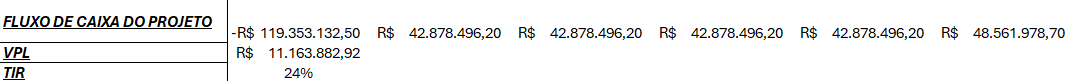
\includegraphics[width=1.0\textwidth]{imagem1.png}
\label{fig:my_label}
\footnotesize{Fonte: Elaborado pelos autores.}
\end{figure}
Em seguida, foi calculado a Taxa Interna de Retorno (TIR), que é uma métrica hipotética que, aplicada a fluxos de caixa, torna as despesas em valor presente iguais aos retornos dos investimentos em valor presente. Ou seja, mensura o quanto o investimento rende ao decorrer do tempo com o VPL igual a zero. 

Caso a TIR seja maior que a TMA, a tomada de decisão é favorável à realização do projeto, já que o retorno interno do projeto é maior que a taxa mínima de atratividade requerida pelos investidores. Se a TIR for menor que a TMA, não é aconselhado que o projeto seja realizado, pois o retorno do investimento é menor que o mínimo esperado deste pelos investidores. 

Para o cálculo da TIR do projeto, utilizou-se a função "TIR" do Excel. Os valores selecionados dentro da fórmula foram todos os fluxos de caixa do projeto, do Ano 0 ao 5. A descrição do cálculo efetuado no Excel pode ser visualizada abaixo:

\begin{verbatim}
=TIR(Fluxo de Caixa do Ano 0:Fluxo de Caixa do Ano 5)
\end{verbatim}

O resultado da operação foi 24\% (Figura 1). Assim sendo, pode-se concluir que a decisão de aprovar o investimento é plausível, já que a TIR é maior que a TMA. Esse resultado evidencia que, ao considerar o Valor Presente Líquido do projeto igual a zero, a TIR é maior que a Taxa de Atratividade Mínima.

\subsubsection{\textbf{Análise do Ponto de Equilíbrio}}
Após a criação do fluxo de caixa do projeto e com a planilha automatizada, faz-se relevante calcular qual a quantidade que deve ser vendido o produto para zerar o lucro, o que chamamos de ponto de equilíbrio contábil, e a quantidade que zera o VPL, o que chamamos de ponto de equilíbrio financeiro ou o econômico.

Para fazermos isso usamos a função de atingir meta do Excel em que definimos qual deve ser a célula que ele deve zerar e qual célula ele deve mudar para que ele o valor dá célula zere.

No ponto de equilíbrio contábil, a quantidade que deve ser vendida para que o lucro líquido seja igual a zero deve ser de 10.825.681 unidades do produto. Isso representa 43\% da quantidade de vendas originalmente estipulada quando foi montado o fluxo de caixa do projeto, no caso, de 25.360.000.

Tal valor não é de grande interesse agora, pois queremos avaliar a viabilidade do projeto, portanto, faz mais sentido olharmos para a quantidade que faz o VPL ser igual a zero. Para tal, repetimos o processo feito para encontrar o ponto de equilíbrio contábil, mas a célula que irá para o valor zero será a célula do VPL. Fazendo isso o valor encontrado pelo atingir meta foi que 22.666.655, esse valor representa 89\% do valor estipulado originalmente de 25.360.000. Esse valor nos mostra que caso a empresa venda 11\% a menos do que ela está estipulando seu projeto irá ter um VPL igual a zero, caso quantidade de venda seja ainda menor que 11\% do valor esperado o projeto terá um VPL negativo, mostrando que é um projeto que não deve ser realizado.

Esse 11\% é uma margem muito baixa para a empresa querer fazer um projeto, qualquer coisa que afete as vendas tem chance de prejudicar esse projeto. Esse é um motivo importante para não executar o projeto.

\subsection{\textbf{Simulação de Monte Carlo no Python}}
Nesta parte, iremos utilizar o Python para criar uma Simulação de Monte Carlo com 100.000 simulações com o objetivo de passar por todas as possíveis situações desse projeto para poder tomar a melhor decisão se vale a pena ou não realizar esse projeto.

Para isso, precisaremos definir certas coisas, como por exemplo, quais os valores que serão simulados, quais as distribuições das variáveis simuladas e quais as variáveis fixas.

No nosso caso, adotamos que a taxa de depreciação, taxa do custo da mercadoria vendida (C.M.V), taxa mínima de atratividade (T.M.A) e a taxa do capital circulante líquido (C.C.L) são as variáveis fixas. Onde a taxa de depreciação é de 20\% sobre o investimento inicial, a taxa de C.M.V é de 79\% sobre a receita, a T.M.A será de 20\% e a taxa de C.C.L será de 5\% sobre o investimento inicial.

Enquanto as variáveis que serão simuladas, elas seguirão ou a distribuição normal ou a distribuição uniforme. As variáveis que seguirão distribuição normal, terão média e desvio padrão. Neste caso, o investimento inicial tem média de R\$113.669.650,00 e desvio padrão de R\$2.500.000,00; na quantidade vendida, ela tem uma média de 25.360.000 e um desvio padrão de 50.000 e o preço tem média de R\$7,70 e desvio padrão de R\$1,50. E a única variável que será simulada e terá distribuição uniforme será o imposto de renda, no qual o valor mínimo é de 34\% e o valor máximo é de 40\%.

Definindo estas variáveis, tanto as fixas quanto as simuladas, podemos começar a simulação de Monte Carlo. Criamos um algoritmo usando a função de iteração “for” para sortear aleatoriamente um valor para as variáveis que serão simuladas e criar o fluxo de caixa do projeto; e a partir delas, calcular o VPL e a TIR de cada simulação, usando a biblioteca numpy\_finance, e salvar esses resultados em dois vetores, um para o VPL e outro para a TIR.

Realizado esse processo, teremos 100.000 valores para o VPL e para a TIR. Projetos realizáveis serão aqueles que possuem um VPL maior que zero, para sabermos qual a probabilidade de realizarmos um projeto e eles nos trazer um retorno, basta dividir quantos projetos possuem VPL maior que zero pelo total de simulações. Em nossos testes, obtivemos valores entre 16\% e 17\% de projetos realizáveis, dentre as 100.000 simulações feitas pelo algoritmo de Monte Carlo. Uma quantidade extremamente baixa de projetos que poderiam dar certo e uma chance extremamente baixa de realizar um projeto e ele dar certo.

Resultando nos seguintes gráficos da distribuição dos VPL’s e TIR’s feitos pela simulação.

\begin{figure}[H]
\centering
\caption{Histograma dos VPL's}
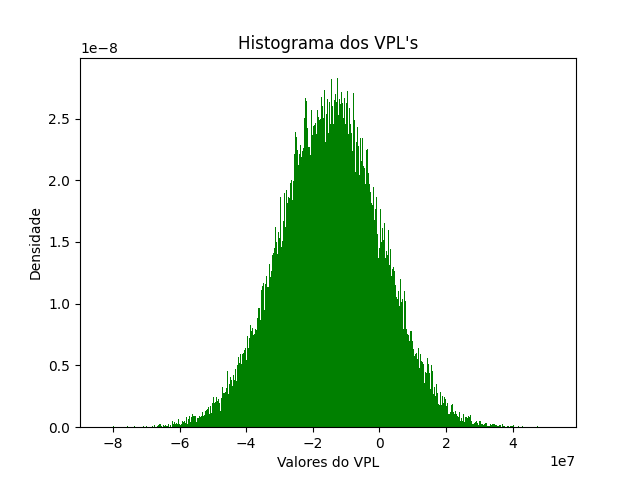
\includegraphics[width=0.5\textwidth]{Histograma dos VPL's.png}
\label{fig:my_label}

\footnotesize{Fonte: Elaborado pelos autores.}
\end{figure}

\begin{figure}[H]
\centering
\caption{Histograma das TIR's}
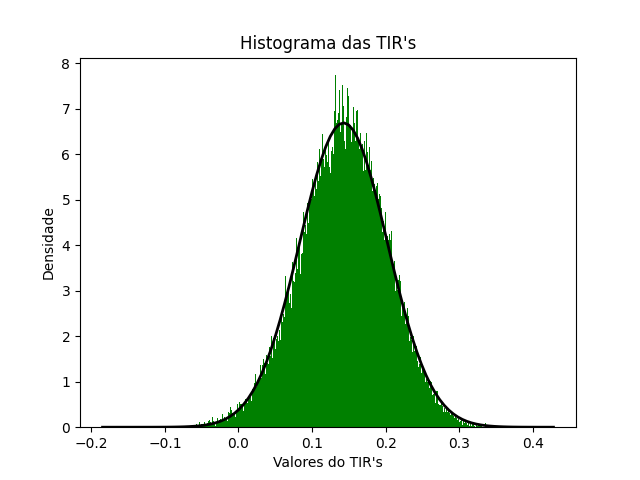
\includegraphics[width=0.5\textwidth]{Histograma das TIR's.png}
\label{fig:my_label}

\footnotesize{Fonte: Elaborado pelos autores.}
\end{figure}

No histograma dos VPL's, somente aqueles valores que estão após o zero representam os projetos que são realizáveis, e esta área acumulada representa os 16\% a 17\% dos projetos realizáveis dentre as 100.000 simulações feitas. A mesma lógica se aplica ao histograma das TIR's, porém começamos a contar os projetos a partir do valor de 0,2, que representa a TMA de 20\%, em que os valores que estão após esse 0,2 representam os projetos realizáveis, e esta área corresponde aos mesmos 16\% a 17\% calculados anteriormente e presentes no histograma dos VPL's.

\subsection{\textbf{Conclusão sobre o Projeto de Investimento}}
Tendo em vista os pontos de equilíbrio, tanto o contábil e principalmente o financeiro/econômico, junto dos resultados apresentados pela simulação de Monte Carlo, chegamos à conclusão de que este é um projeto que não deve ser realizado devido a baixa chance de ele ter sucesso.

\newpage
\begin{thebibliography}{9}
\section{Bibliografia Consultada}
\bibitem{caetano2021} 
CAETANO, Marco Antonio L. 
\textit{Python e mercado financeiro}. 
[Digite o Local da Editora]: Editora Blucher, 2021. E-book. ISBN 9786555062410. 
Disponível em: \href{https://app.minhabiblioteca.com.br//books/9786555062410/}{https://app.minhabiblioteca.com.br//books/9786555062410/}. 
Acesso em: 05 nov. 2023.

\bibitem{camil2022} 
CAMIL. 
\textit{Demonstração contábil 2022}. 
Disponível em: \href{https://api.mziq.com/mzfilemanager/v2/d/65f65acb-ad9a-44b1-a3d5-620b6199a637/d37a81aa-c092-93bc-b378-38e4bc77c532?origin=2}{https://api.mziq.com/mzfilemanager/v2/d/65f65acb-ad9a-44b1-a3d5-620b6199a637/d37a81aa-c092-93bc-b378-38e4bc77c532?origin=2}. 
Acesso em: 05 nov. 2023.

\bibitem{kiyokawa2023} 
AULA DE MONTE CARLO USANDO CRYSTAL BALL NO EXCEL. 
Direção de Fabricio Kiyokawa. Produção de Fabricio Kiyokawa.
Disponível em: \href{https://1drv.ms/v/s!AqjSkj4Rz9gFg69wpOPvXqm9GuFhkA?e=UtF1oL}{https://1drv.ms/v/s!AqjSkj4Rz9gFg69wpOPvXqm9GuFhkA?e=UtF1oL}. 
Acesso em: 5 nov. 2023.
\end{thebibliography}

\newpage
\appendix
\section{Código Python para Simulação de Monte Carlo}
\begin{verbatim}
#%%Sobre este Trabalho
"""
Este trabalho se trata do APS de Finanças I, em que simularemos o
VPL de um projeto, mas usaremos do Python para realizar a Simulação de
Monte Carlo para avaliar a viabilidade da realização do projeto.
"""

#Integrantes
"""
Beatriz Emi Ueda (beatrizeu@al.insper.edu.br),  
Beatriz Fernandes da Silva (beatrizfs1@al.insper.edu.br),  
Gabriela Abib (gabrielaa6@al.insper.edu.br),  
Hicham Munir Tayfour (hichamt@al.insper.edu.br),  
Júlia de Aquino Rocha (juliaar1@al.insper.edu.br),  
Raynnara Silva de Freitas Gurgel (raynnarasf@al.insper.edu.br).  
"""

#Empresa escolhida: Camil (CAML3.SA)

#%% Bilbliotecas à serem usadas para a simulação de Monte Carlo
import numpy_financial as fin
import numpy as np
import matplotlib.pyplot as fig

#%% Simulação de Monte Carlo

#Premissas
"""
Vamos adotar a distribuição normal e uniforme como padrão da simulação,
onde a normal será usada 
para grande parte da simulação e a distribuição uniforme será usada
somente para o intervalo de Imposto de Renda .
Projeto Terá uma Duração de 5 anos
"""

#Variaveis e Simulção
Simulações=int(100000)
VPL=np.zeros(Simulações)
TIR=np.zeros(Simulações)

"Variáveis Fixas"
Taxa_Depreciação=float(0.2)
Taxa_CMV=float(0.79)
TMA=float(0.2)
Taxa_CCL=float(0.05)

"Variáveis a Serem Simuladas"
MediaInvestimento=int(113669650)
DesvioInvestimento=int(2500000)
MediaQuantidade=int(25360000)
DesvioQuantidade=int(50000)
MediaPrecoUnitario=float(7.70)
DesvioPrecoUnitario=float(1.50)
IR_Max=float(0.4)
IR_Min=float(0.34)

"Simulação"
for i in range(Simulações):
    #Distribuição das Variáveis Aleatórias 
    Investimento=round(np.random.normal(MediaInvestimento,DesvioInvestimento),2)
    Quantidade=round(np.random.normal(MediaQuantidade,DesvioQuantidade),2)
    Preco=round(np.random.normal(MediaPrecoUnitario,DesvioPrecoUnitario),2)
    IR=np.random.uniform(IR_Min,IR_Max)
    #Montagem do Fluxo De Caixa 
    Receita=Quantidade*Preco
    CMV=Taxa_CMV*Receita
    Depreciação=Taxa_Depreciação*Investimento
    LAJIR=Receita-(CMV+Depreciação)
    Imposto=LAJIR*IR
    NOPAT=LAJIR-Imposto
    FCO=NOPAT+Depreciação
    CCL=Investimento*Taxa_CCL
    FxCx0=-(Investimento+CCL)
    FxCx5=FCO+CCL
    FxCxProjeto=np.array([FxCx0,FCO,FCO,FCO,FCO,FxCx5])
    VPL[i]=fin.npv(TMA,FxCxProjeto)
    TIR[i]=fin.irr(FxCxProjeto)

#Quais os Projetos Viáveis (VPL>0)
Realizavel=VPL[VPL>0]
NumRealizaveis=len(Realizavel)

ProbabilidadeRealizável=round(100*(NumRealizaveis/Simulações),2)
print("A probabilidade da empresa realizar o projeto ,
ou seja, o projeto possuir um VPL maior que zero é de  ",ProbabilidadeRealizável,"%")


#Representções Gráficas do VPL e da TIR
fig.figure()
fig.hist(VPL, bins=1000, color='green', density=True)
fig.title("Histograma dos VPL's")
fig.xlabel("Valores do VPL")
fig.ylabel("Densidade")

fig.figure()
fig.hist(TIR, bins=1000, color='green',density=True)
fig.title("Histograma das TIR's")
fig.xlabel("Valores do TIR's")
fig.ylabel("Densidade")
\end{verbatim}

\end{document}
